% Note: this need to be compiled twice! 
\documentclass[11pt,twocolumn,landscape,a4paper,notitlepage]{article}

% Packages
\usepackage{calc}			% for length arithmetic.
\usepackage[twocolumn, top=1.0cm, bottom=1.0cm, left=1.0cm, right=1.0cm, voffset=0cm, hoffset=0cm, headsep=0.2cm, headheight=13.6pt, footskip=\headsep + \headheight, columnsep=1.25cm]{geometry}
\usepackage{babel}
\usepackage{listings} 				% for code snippets.
\usepackage{fancyhdr}				% for headers and footers.
\usepackage{etoolbox}				% for the \maketitle hack.
\usepackage{array}					% for table column specifications.
\usepackage{graphicx}				% for table resize.
\usepackage{booktabs}				% for tables.
\usepackage{xtab}					% for multiple pages tables.
\usepackage[hidelinks]{hyperref}	% for click-able toc
\usepackage{amsmath}
\usepackage{graphicx}
\usepackage{ragged2e}
\usepackage{xcolor}

% Dibujar grafos
\usepackage{tikz} 

\lstnewenvironment{code}
    {%\lstset{	numbers=none, frame=lines, basicstyle=\small\ttfamily, }%
    \csname lst@SetFirstLabel\endcsname}
    {\csname lst@SaveFirstLabel\endcsname}
% We create some new table columns types.
\newcolumntype{L}[1]{>{\raggedright\let\newline\\\arraybackslash\hspace{0pt}}m{#1-2\tabcolsep- 1.25\arrayrulewidth}}
\newcolumntype{C}[1]{>{\centering\let\newline\\\arraybackslash\hspace{0pt}}m{#1-2\tabcolsep- 1.25\arrayrulewidth}}
\newcolumntype{R}[1]{>{\raggedleft\let\newline\\\arraybackslash\hspace{0pt}}m{#1-2\tabcolsep- 1.25\arrayrulewidth}}

% We make visible heder's and footer's ruler.
\renewcommand{\headrulewidth}{0.5pt}
\renewcommand{\footrulewidth}{0.5pt}
\renewcommand{\columnseprule}{0.5pt}

% To display the footer and header on the first page.
\fancypagestyle{plain}
{
	\fancyhf{}
	\rhead{piashi piashii}
	\lhead{UTN FRRO - hola}
	\rfoot{P\'agina \thepage}
}
\pagestyle{plain}

% and for the rest of the pages.
\fancyhf{}
\rhead{\leftmark}
\lhead{UTN FRRO - hola}
\rfoot{P\'agina \thepage}

% We use Courier font to make bold keywords possible.
\renewcommand{\ttdefault}{pcr}

\usepackage{xcolor}
\definecolor{commentgreen}{RGB}{2,112,10}

% Listing code style
\lstdefinestyle{codestyle}{
	basicstyle=\scriptsize\ttfamily,
    keywordstyle=\bfseries,
    emph={int,char,double,float,unsigned,void,bool},
    emphstyle=\bfseries,
    breakatwhitespace=false,
    breaklines=true,
    captionpos=b,
    keepspaces=false,
    numbers=left,
    numberstyle=\tiny\ttfamily,
    numbersep=5pt,
    frame=single,
    framesep=3pt,
    showspaces=false,
    showstringspaces=false,
    showtabs=false,
    tabsize=2,
    commentstyle=\color{commentgreen}, % comment color
    keywordstyle=\color{blue}, % keyword color
    stringstyle=\color{red} % string color
}
\lstset{style=codestyle}

% To dislpay the title on one column 
\makeatletter
% Remove the brackets so LaTeX sees \twocolumn\@maketitle
\patchcmd{\maketitle}{[\@maketitle]}{\@maketitle}{}{}
% Remove the vertical shift from the title 
\patchcmd{\@maketitle}{\null\vskip2em\begin{center}}{\vspace*{0pt}\nointerlineskip\begingroup\centering}{}{}
% In the final part we must remove \end{center}
\patchcmd{\@maketitle}{\end{center}\par}{\par\endgroup}{}{}
\makeatother


% Information
\author{UTN FRRO - HOLA}
\title{Notebook}
\date{2024}


\begin{document}
\maketitle
\tableofcontents
\newpage

% Here we include each section of this notebook from external files.
\newpage
\section{Basics}

\subsection{Template}
\lstinputlisting[language=C++]{secciones/basics/template.cpp}

\subsection{Compilation}
\begin{lstlisting}
g++ -DEBUG <ej>.cpp -o a && time ./a
\end{lstlisting}
\newpage

\newpage
\section{Estructuras}

\subsection{vector}
\begin{center}
    \begin{tabular}{||l|l|l||}
        \hline
        \textbf{Función}          & \textbf{Explicación}                              & \textbf{O} \\ \hline
        (constructor)             & Construct vector                                  & O(n)                 \\ \hline
        (destructor)              & Vector destructor                                 & O(n)                 \\ \hline
        operator=                 & Assign content                                    & O(n)                 \\ \hline
        begin                     & Return iterator to beginning                      & O(1)                 \\ \hline
        end                       & Return iterator to end                            & O(1)                 \\ \hline
        rbegin                    & Return reverse iterator to reverse beginning      & O(1)                 \\ \hline
        rend                      & Return reverse iterator to reverse end            & O(1)                 \\ \hline
        cbegin                    & Return const\_iterator to beginning               & O(1)                 \\ \hline
        cend                      & Return const\_iterator to end                     & O(1)                 \\ \hline
        crbegin                   & Return const\_reverse\_iterator to reverse beginning  & O(1)             \\ \hline
        crend                     & Return const\_reverse\_iterator to reverse end    & O(1)                 \\ \hline
        size                      & Return size                                       & O(1)                 \\ \hline
        resize                    & Change size                                       & O(n)                 \\ \hline
        empty                     & Test whether vector is empty                      & O(1)                 \\ \hline
        operator[]                & Access element                                    & O(1)                 \\ \hline
        at                        & Access element                                    & O(1)                 \\ \hline
        front                     & Access first element                              & O(1)                 \\ \hline
        back                      & Access last element                               & O(1)                 \\ \hline
        assign                    & Assign vector content                             & O(n)                 \\ \hline
        push\_back                & Add element at the end                            & O(1) \\ \hline
        pop\_back                 & Delete last element                               & O(1)                 \\ \hline
        insert                    & Insert elements                                   & O(n)                 \\ \hline
        erase                     & Erase elements                                    & O(n)                 \\ \hline
        swap                      & Swap content                                      & O(1)                 \\ \hline
        clear                     & Clear content                                     & O(n)                 \\ \hline
        emplace                   & Construct and insert element                      & O(1) \\ \hline
        emplace\_back             & Construct and insert element at the end           & O(1) \\ \hline
    \end{tabular}
\label{tab:vector_member_functions_complexity}
\end{center}

\newpage
\subsubsection{emplace}
\begin{lstlisting}[language=C++]
vector<int> myvector = {10,20,30};

auto it = myvector.emplace ( myvector.begin()+1, 100 );
myvector.emplace ( it, 200 );
myvector.emplace ( myvector.end(), 300 );

for (auto& x: myvector)
    cout << ' ' << x;
// 10 200 100 20 30 300
\end{lstlisting}

\subsubsection{resize}
Resizes the container so that it contains n elements. \\
\lstinline[language=C++]{void resize (size_type n, const value_type& val);}
\begin{lstlisting}[language=C++]
vector<int> myvector;
for (int i=1; i<10; i++) myvector.push_back(i);

myvector.resize(5);
myvector.resize(8, 100);
myvector.resize(12);

for (int i=0;i<myvector.size();i++)
    cout << ' ' << myvector[i];
//  1 2 3 4 5 100 100 100 0 0 0 0
\end{lstlisting}

\subsubsection{assign}
Assigns new contents to the vector, replacing its current contents, and modifying its size accordingly. \\
\lstinline[language=C++]{void assign (size_type n, const value_type& val);

\begin{lstlisting}[language=C++]
vector<int> first;
vector<int> second;
vector<int> third;

first.assign (7,100);             // 7 ints with a value of 100

vector<int>::iterator it;
it=first.begin()+1;

second.assign (it,first.end()-1); // the 5 central values of first

int myints[] = {1776,7,4};
third.assign (myints,myints+3);   // assigning from array.

first.size() // -> 7
second.size() // -> 5
third.size()) // -> 3

\end{lstlisting}



\subsection{unordered set}
\begin{center}
    \begin{tabular}{||l|l|l||}
        \hline
        \textbf{Función}         & \textbf{Explicación}                               & \textbf{O} \\ \hline
        (constructor)            & Construct unordered\_set                          & -    \\ \hline
        (destructor)             & Destroy unordered\_set                            & -    \\ \hline
        operator=                & Assign content                                    & O(n) \\ \hline
        empty                    & Test whether container is empty                   & O(1) \\ \hline
        size                     & Return container size                             & O(1) \\ \hline
        max\_size                & Return maximum size                               & O(1) \\ \hline
        begin                    & Return iterator to beginning                      & O(1) \\ \hline
        end                      & Return iterator to end                            & O(1) \\ \hline
        find                     & Get iterator to element                           & O(n) \\ \hline
        count                    & Count elements with a specific key                & O(n) \\
                                 & Returns 0 or 1                                    & \\ \hline
        equal\_range             & Get range of elements with a specific key         & O(n) \\ \hline
        emplace                  & Construct and insert element                      & O(n) \\ \hline
        emplace\_hint            & Construct and insert element with hint            & O(n) \\ \hline
        insert                   & Insert elements                                   & O(n) \\ \hline
        erase                    & Erase elements                                    & O(n) \\ \hline
        clear                    & Clear content                                     & O(n) \\ \hline
        swap                     & Swap content                                      & O(1) \\ \hline
        reserve                  & Request a capacity change                         & O(n) \\ \hline
        key\_eq                  & Get key equivalence predicate                     & O(1) \\ \hline
    \end{tabular}
    \label{tab:set_member_functions_complexity}
\end{center}
\newpage

\begin{lstlisting}[language=C++]
unordered_set<int> s;
s.insert(3);
s.insert(5);
s.erase(3);
s.count(3); // -> 0
s.count(5); // -> 1
\end{lstlisting}


\subsection{Iterators}
\begin{lstlisting}[language=C++]
sort(v.begin(), v.end());
reverse(v.begin(), v.end());
random_shuffle(v.begin(), v.end());

sort(v.begin(), v.end(), sortbysec);
\end{lstlisting}

sort complexity = $O(N log_2 N)$.

Ordenar un vector de pair por su segunda componente
\begin{lstlisting}[language=C++]
vector<pair<int, int>> v;

bool sortbysec(const pair<int,int> &a, const pair<int,int> &b){
	return (a.second < b.second);
}
\end{lstlisting}

También es posible ordenar un array normal:
\begin{lstlisting}[language=C++]
sort(a, a+n);
reverse(a, a+n);
random_shuffle(a, a+n)
\end{lstlisting}

\subsection{Indexed Set}
\lstinputlisting[language=C++][secciones/estructuras/indexedSet.cpp]

\subsection{Segment Tree}
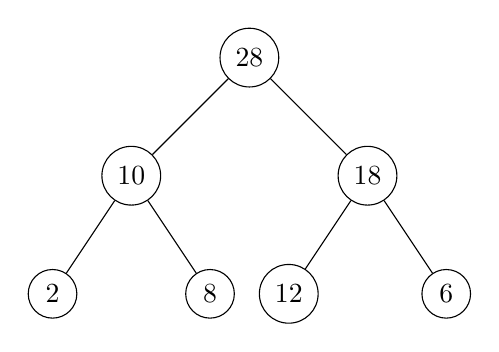
\begin{tikzpicture}[main/.style = {draw, circle}]
    % Nivel 1
    \node[main] (1) at (0,0) {28};

    % Nivel 2
    \node[main] (2) at (-1.5,-1.5) {10};
    \node[main] (3) at (1.5,-1.5) {18};

    % Nivel 3
    \node[main] (4) at (-2.5,-3) {2};
    \node[main] (5) at (-0.5,-3) {8};
    \node[main] (6) at (0.5,-3) {12};
    \node[main] (7) at (2.5,-3) {6};

    % Conexiones
    \draw (1) -- (2);
    \draw (1) -- (3);
    \draw (2) -- (4);
    \draw (2) -- (5);
    \draw (3) -- (6);
    \draw (3) -- (7);
\end{tikzpicture}

\lstinputlisting[language=C++]{secciones/estructuras/segment-tree.cpp}
\subsection{Array}
\lstinputlisting[language=C++]{secciones/estructuras/array.cpp}
\subsection{BitSet}
\begin{center}
    \begin{tabular}{||l|l|l||}
    \hline
    \textbf{Función}    & \textbf{Explicación}          & \textbf{O} \\ \hline

    \textbf{Template parameters} & & \\ \hline
        N               & número de bits             & O(1) \\ \hline

    \textbf{Member functions} & & \\ \hline
    (constructor) & construye el `bitset` & O(N) \\ \hline

    \textbf{Element access} & & \\ \hline
    operator[]          & accede a un bit específico    & O(1) \\ \hline
    all, any, none      & todos, algún o ningún bit está en true  & O(N) \\ \hline
    count               & número de bits establecidos en true     & O(N) \\ \hline
    size                & número de bits que contiene & O(1) \\ \hline

    \textbf{Modifiers} & & \\ \hline
        operator\&=  & & \\
        operator|= & & \\
        operator\textasciicircum= & & \\
        operator\textasciitilde= & & \\
        operator<<= & & \\
        operator>>= & & \\
        operator<< & & \\
        operator>> & & O(N) \\ \hline
        set() & pone todos los bits en el valor dado        & O(N) \\
        set(int pos) &                                      & O(1) \\ \hline
        reset() & establece bits en `false`                 & O(N) \\
        reset(int pos) &                                    & O(1) \\ \hline
        flip() & alterna los valores de los bits            & O(N) \\
        flip(int pos) & &O(1) \\ \hline

    \textbf{Conversions} & & \\ \hline
    to\_string & representación en cadena
    \end{tabular}
\end{center}

\newpage

\newpage
\section{Grafos}

\subsection{Recorrer Grafos}
Dado un Grafo como lista de adjacencias

\begin{lstlisting}[language=C++]
#include <bits/stdc++.h>
#define MAXN 100000
using namespace std;

vector<int> G[MAXN];
bool visited[MAXN];
\end{lstlisting}

Podemos recorrerlo con DFS o con BFS.

\subsubsection{DFS}
\lstinputlisting[language=C++]{secciones/grafos/dfs.cpp}

\subsubsection{BFS}
\lstinputlisting[language=C++]{secciones/grafos/bfs.cpp}
\newpage

\subsection{Camino Mínimo}

\subsubsection{Bellman-Ford}
El algoritmo de Bellman-Ford encuentra el camino desde un nodo de origen a todos los nodos del grafo. \\
\textbf{Complejidad = O(nm)}

\lstinputlisting[language=C++]{secciones/grafos/bellman-ford.cpp}
\subsubsection{Ciclos negativos}
El algoritmo es capaz de detectar ciclos negativos. Para eso Se debe correr una vez m'as
\newpage

\subsubsection{Dijkstra}
El algorimo necesita que todos los pesos sean > 0 \\
\textbf{Complejidad = O(n + m log m)}
\lstinputlisting[language=C++]{secciones/grafos/dijkstra.cpp}
\newpage
\subsubsection{Floyd-Warshall}
\lstinputlisting[language=C++]{secciones/grafos/floyd.cpp}

\newpage

\newpage
\section{Geometria}

\subsection{Punto}
\lstinputlisting[language=C++]{secciones/geometria/pto.cpp}

\subsection{Line}
\lstinputlisting[language=C++]{secciones/geometria/line.cpp}

\subsection{Segment}
\lstinputlisting[language=C++]{secciones/geometria/segment.cpp}

\subsection{Circle}
\lstinputlisting[language=C++]{secciones/geometria/circle.cpp}

\newpage

\section{Utils}

\subsection{Binary Search}
\lstinputlisting[language=C++]{secciones/utils/bs.cpp}

\subsection{Sort}
Ordenar un vector de pair por su segunda componente
\begin{lstlisting}[language=C++]
vector<pair<int, int>> v;

bool sortbysec(const pair<int,int> &a, const pair<int,int> &b){
	return (a.second < b.second);
}

sort(v.begin(), v.end(), sortbysec);
\end{lstlisting}
\subsection{Cout para doubles}
\begin{lstlisting}[language=C++]
cout << fixed << setprecision(20) << ans << endl;
\end{lstlisting}
\subsection{Prev permutation}
\lstinputlisting[language=C++]{secciones/utils/prevpermutation.cpp}
\subsection{MO}
\lstinputlisting[language=C++]{secciones/utils/mo.cpp}

\subsection{Criba}
Nros primos hasta maxp
\lstinputlisting[language=C++]{secciones/utils/criba.cpp}

\subsection{Subconjuntos}
Subconjuntos distintos de un conjunto
\lstinputlisting[language=C++]{secciones/utils/Subconjuntos.cpp}

\subsection{Propiedades del Bitwise XOR ($\oplus$)}
\begin{enumerate}
    \item \textbf{Identidad:} 
    \[
    a \oplus 0 = a
    \]

    \item \textbf{Autoinversión:} 
    \[
    a \oplus a = 0
    \]

    \item \textbf{Conmutativa:} 
    \[
    a \oplus b = b \oplus a
    \]

    \item \textbf{Asociativa:} 
    \[
    (a \oplus b) \oplus c = a \oplus (b \oplus c)
    \]

    \item \textbf{Autoeliminación:} 
    \[
    a \oplus a \oplus b = 0 \oplus b = b
    \]

    \item \textbf{Uso práctico: Encontrar elemento único} \\
    Si todos los elementos de un conjunto aparecen dos veces excepto uno:
    \[
    x_1 \oplus x_2 \oplus \dots \oplus x_n = \text{elemento único}
    \]
\end{enumerate}

\newpage




\end{document}
